\section{DETAILED DESIGN AND REALIZATION}

AtlantikSolar (Figs. \ref{fig:AtlantikSolarCollage} and \ref{fig:CAD_AtlantikSolarFull}) is a solar-powered Low-Altitude Long-Endurance(LALE) Unmanned Aerial Vehicle designed for perpetual flight at $\varphi=45°$ geographical latitude from April 21\textsuperscript{st} to August 21\textsuperscript{st}. It was designed and built at ETH Zurich as a lightweight high aspect ratio airplane to achieve minimum sink rate. Although its design is mostly dictated by the requirement for low power consumption, it does provide the option to use visual\&infrared sensor systems and on-board computation ressources in an autonomous operation mode for use in search and rescue or industrial inspection applications. The airplane design is summarized in table \ref{tab:DetailedDesignParameters}. Figure \ref{fig:AtlantikSolar_SystemOverview} presents an overview over the aircraft components topology.

\begin{figure}[tb]
    \centering
    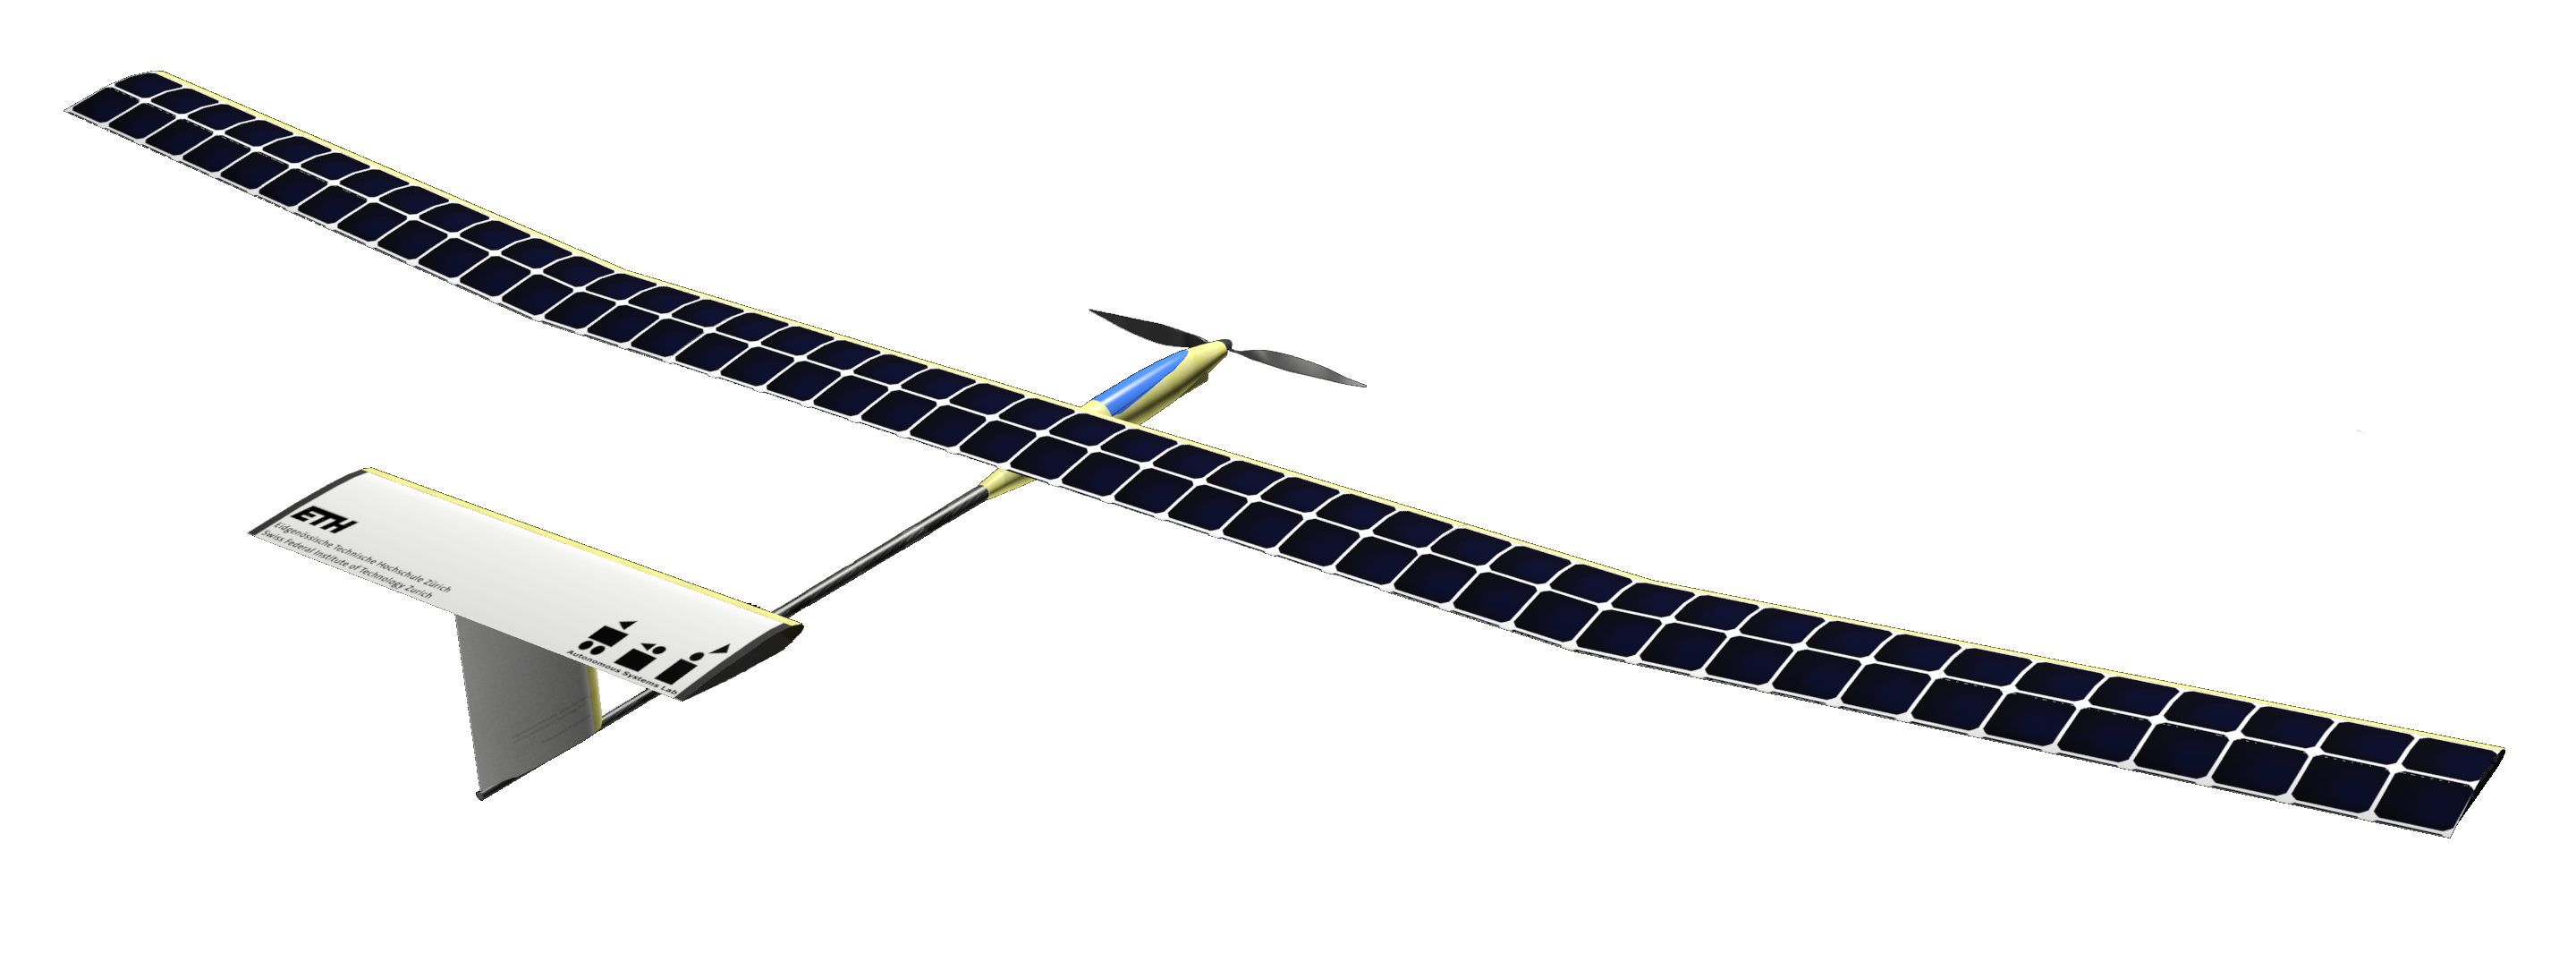
\includegraphics[width=\linewidth]{images/6_CAD_AtlantikSolarFull}
    \caption{The AtlantikSolar UAV features a conventional T-tail configuration with 1 motor, two ailerons, an all-moving elevator and a rudder for actuation.}
    \label{fig:CAD_AtlantikSolarFull}
\end{figure}

\begin{table}
\label{tab:DetailedDesignParameters}
\caption{AtlantikSolar design characteristics}
\begin{center}
\begin{tabular}{l l}
Wing span & 5.65$\unit{m}$\\
\hline Wing chord& 0.305$\unit{m}$\\
\hline Length& \\
\hline Height&\\
\hline Mass& 7.36$\unit{kg}$\\
\hline Battery mass& 3.52$\unit{kg}$\\
\hline Wing loading&4.28$\unitfrac{kg}{m^2}$\\
\hline Stall speed& 8.1$\unitfrac{m}{s}$ TBD\\
\end{tabular}
\end{center}
\end{table}

\subsection{UAV Platform Design}
\subsubsection{Airframe and hardware}

The structure of AtlantikSolar is built in a traditional rib-spar construction method. The wing (Fig. \ref{fig:CAD_AtlantikSolarStructure}) consists of an inner cylindrical carbon-fibre spar to resist torsional wing loads. Four carbon-fibre belts of trapezoidal and laterally-varying cross-section are located around the spar to optimally resist bending loads and to provide maximum wing stiffness to protect the solar cells on the wings. Equally-spaced balsa-wood ribs and the kevlar-reinforced wing leading edge provide structural support for the non-load-carrying outer wing surface. The horizontal and vertical tail planes are constructed in a similar fashion.

\begin{figure}[tb]
    \centering
    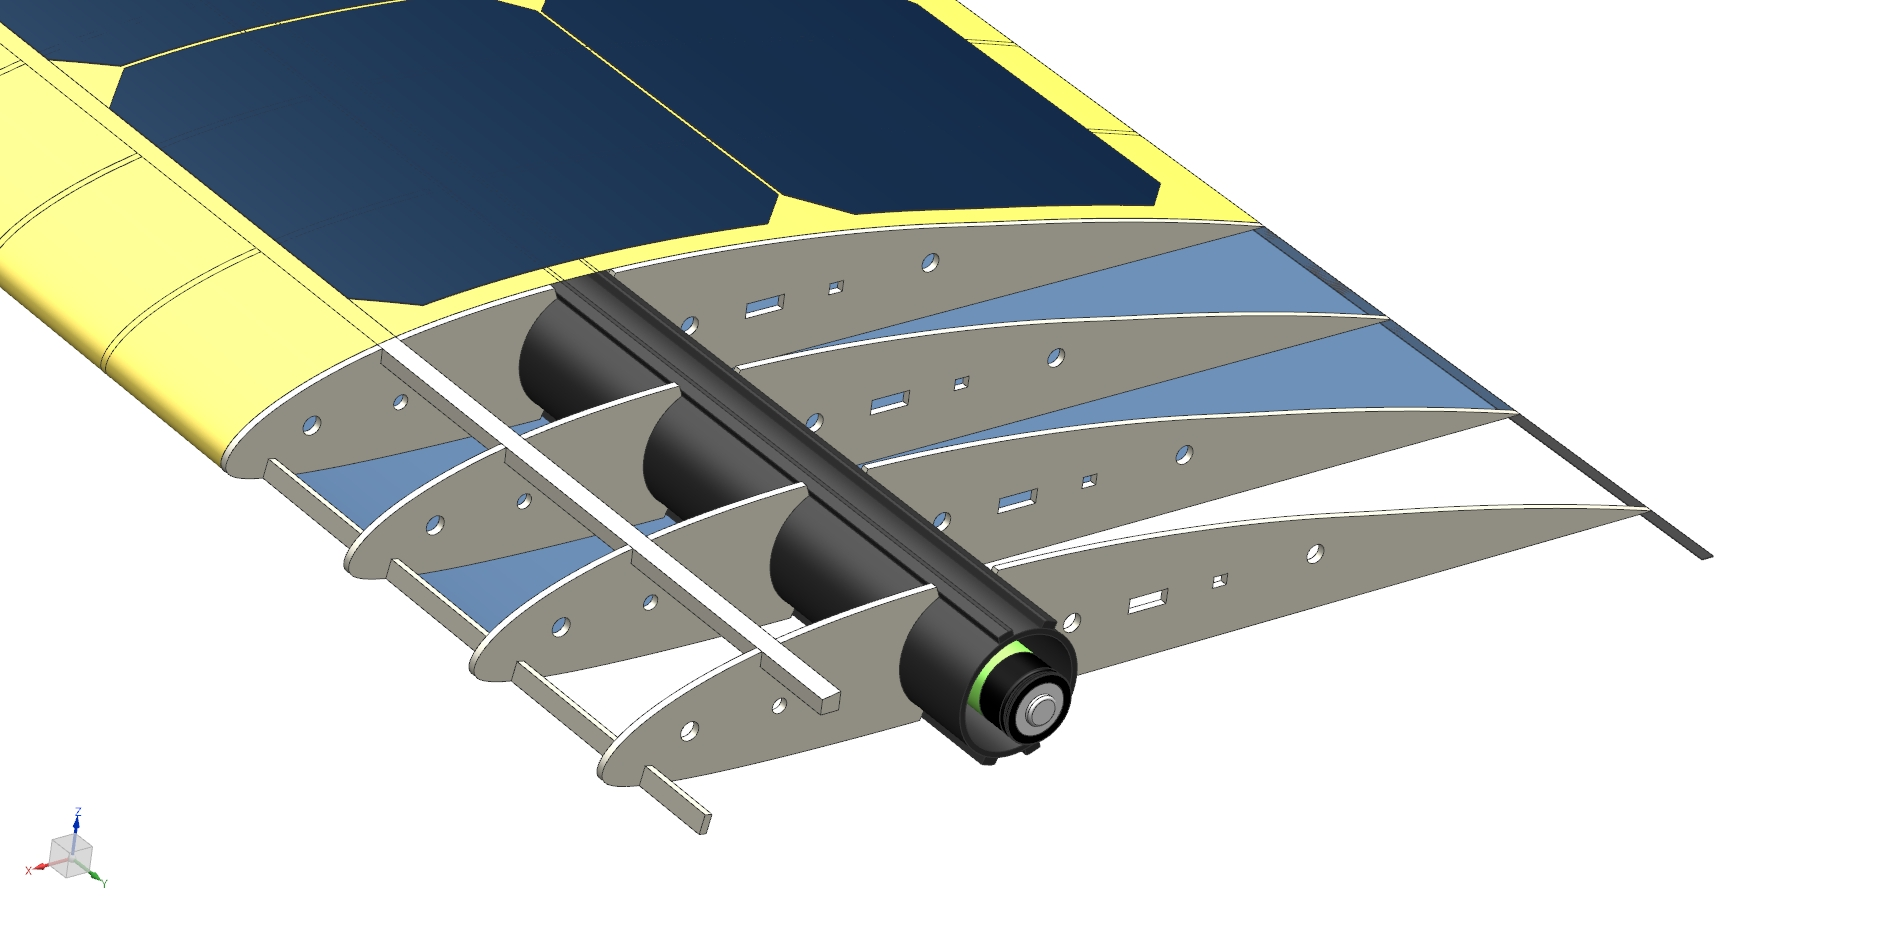
\includegraphics[width=\linewidth]{images/7_CAD_AtlantikSolarStructure}
    \caption{AtlantikSolar's wing structure, integrated batteries and solar cells.}
    \label{fig:CAD_AtlantikSolarStructure}
\end{figure}

The cylindrical wing spar contains a total of 60 cylindrical Lithium-Ion battery cells to optimally distribute the battery mass in a ``span loader'' concept. An additional 12 batteries can be added inside the outer wings to optimize the aircraft for a specific application. The Li-Ion cells are Panasonic NCR18650b high energy density (243Wh/kg) industrial cells.They are connected in a 6S (22.2V) configuration and provide $E_{bat,max}=850Wh$ at $m_{bat}=3.5kg$. The solar modules are seamlessly embedded into the upper wing surface to avoid premature flow separation. They feature a total of 88 SunPower C60 cells with a measured module-level efficiency of $\eta_{sm}=0.20$, an areal density of $k_{sm}=590g/m^2$ and a maximum power output of 275W at $\varphi=45°$ on June21\textsuperscript{st}. Modules featuring SunPower E60 cells with a verified module-level efficiency of $eta_sm=0.23$ are currently being integrated.

The propulsion system features a foldable carbon-fibre propeller with $D=66cm$ and 60cm pitch that was specifically developed to achieve $\eta_{propeller}=82\%$ at the nominal operating point of $F_{propeller}=2.4N$ at $v=8.5\unitfrac{m}{s}$. The propeller is driven by a 5:1 reduction-ratio planetary gearbox, a RS-E Strecker 260.20 brushless DC motor with $k_V=570RPM/V$ and a Kontronik Koby 55 LV motor controller. The propulsion system delivers a maximum electrical power of $P_{prop,max}=450W$. The actuation system consists of four Volz DA-15N servos that drive the two ailerons, the all-moving elevator and the rudder. To guarantee reliable multi-day flight, the Volz actuators were successfully bench-tested throughout a simulated continuous 30-day flight \cite{DellaCa_BT}.
%mention wind tunnel, lab motor test stand tests? Only if space left...

\subsubsection{Avionics}

The AtlantikSolar avionics topology is shown in Fig. \ref{fig:AtlantikSolar_SystemOverview} and an integration snapshot is presented in Fig. \ref{fig:9_CAD_AtlantikSolarAvionics}. Multiple sensors are centered around a Pixhawk PX4 Autopilot - an open source and open hardware project initiated at ETH Zurich - with a Cortex M4F microprocessor running at 168Mhz and featuring 192kB RAM. For state estimation (section XXX), an ADIS 16448 10-axis Inertial Measurement Unit (IMU), a u-Blox LEA-6H GPS receiver, and a Sensirion SDP600 differential pressure (i.e. airspeed) sensor are used. The SDP600 airspeed sensor has been chosen due to its low relative error of less than 5\% at airspeeds of 8m/s, which is necessary to closely control the airspeed to the airspeed with minimum required power $P_{out}$. Commands are received through a 433Mhz telemetry link for medium ranges, or through a long-range IRIDIUM-based satellite communication link that also serves as a backup in case of primary telemetry link failure. The airplane implements a fully manual RC-command fallback mode in case of a severe autopilot failure. Night operations are possible due to four on-board high-power LEDs.

\begin{figure}[tb]
    \centering
   % 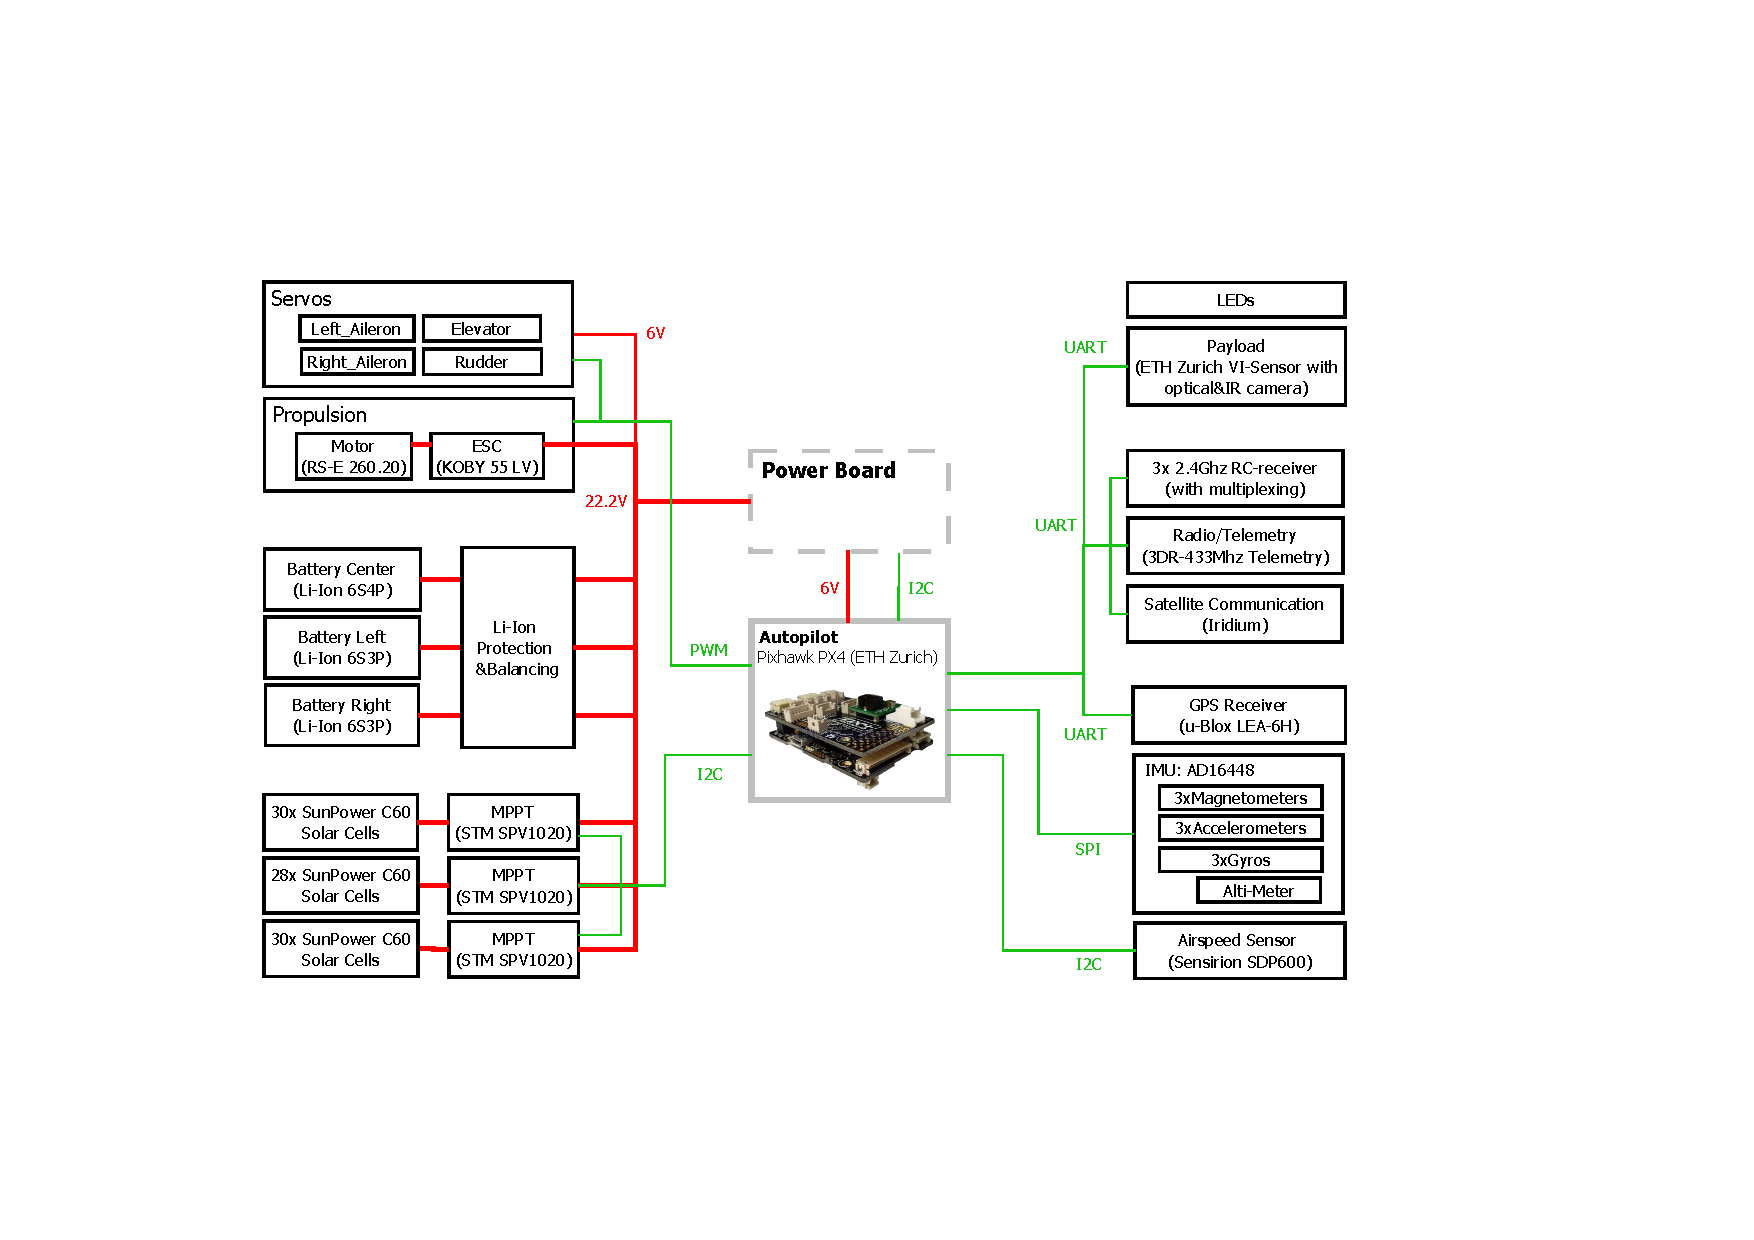
\includegraphics[width=\linewidth]{images/8_AtlantikSolar_Avionics}
     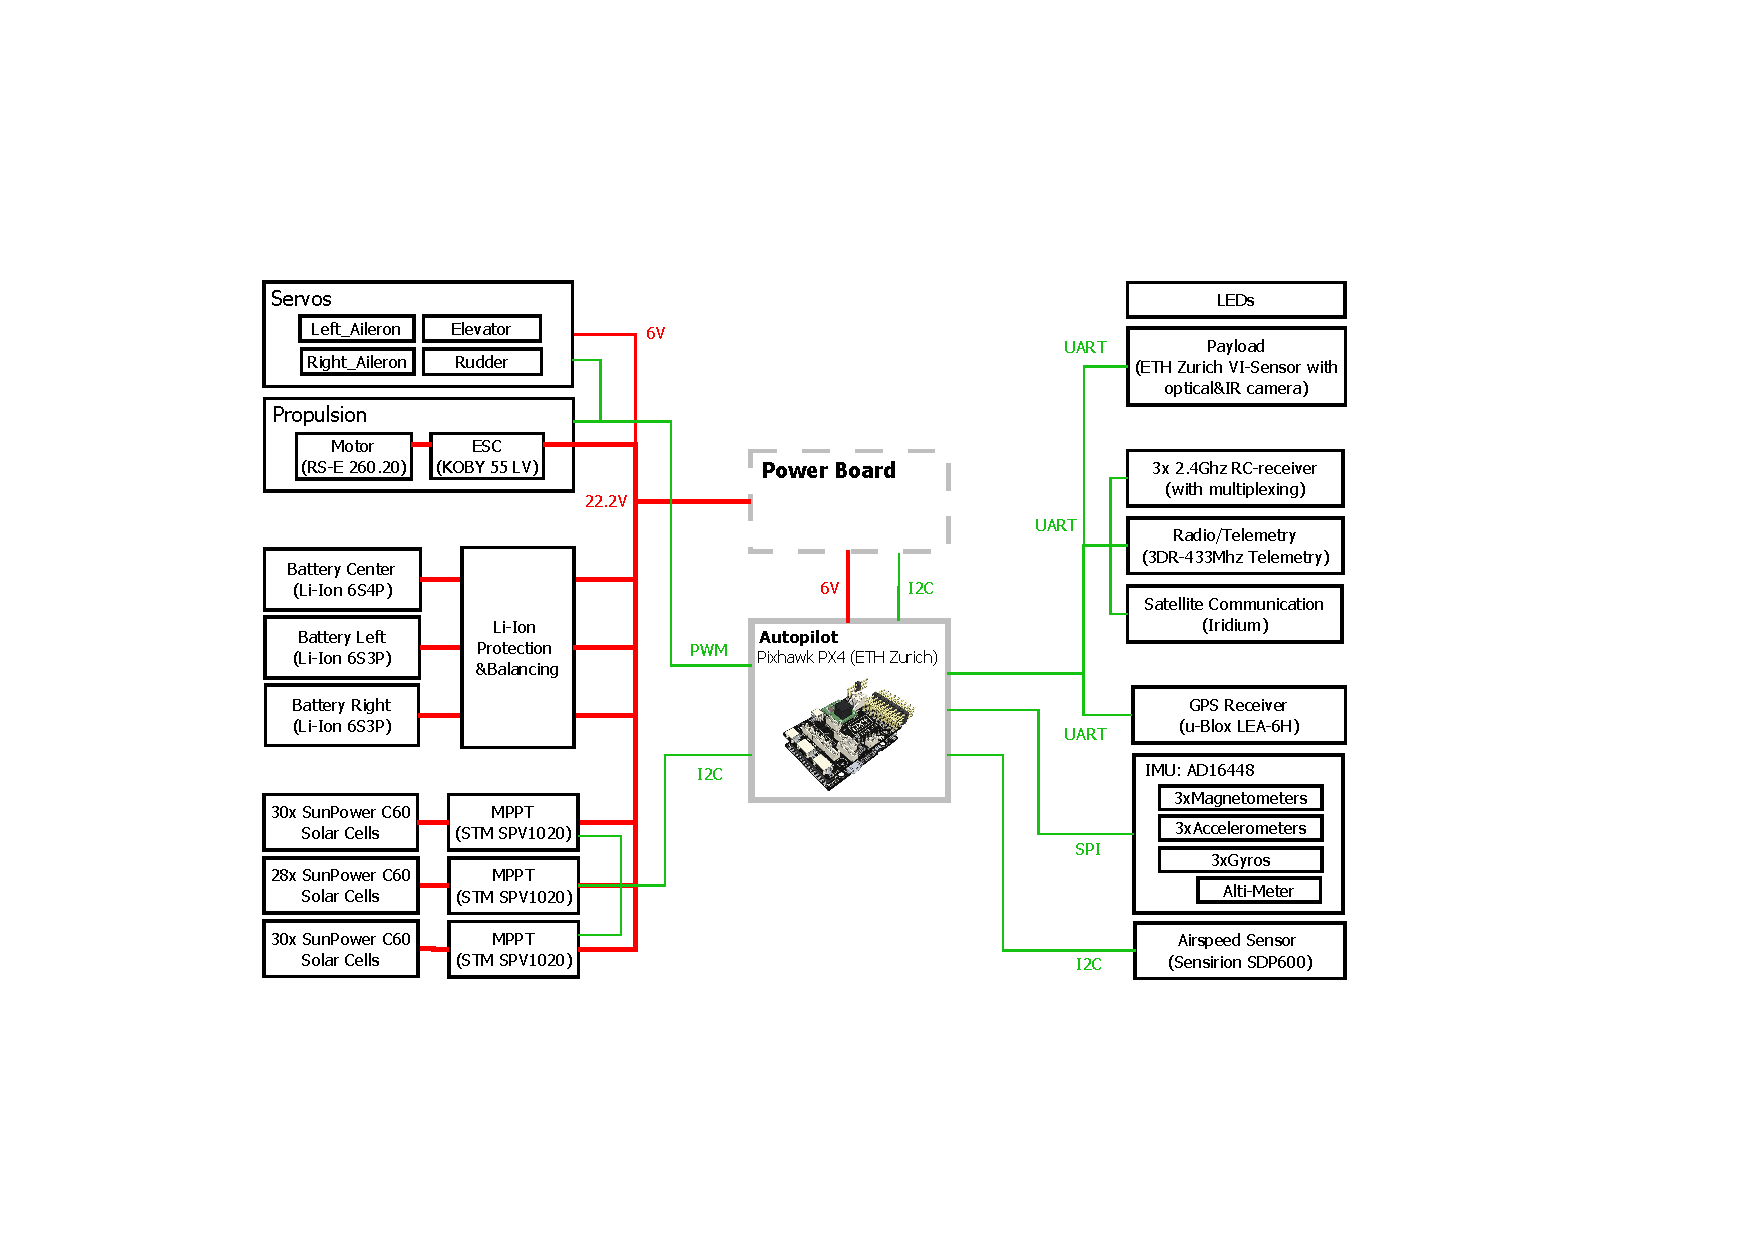
\includegraphics[width=\linewidth]{images/8b_AtlantikSolar_Avionics}
    \caption{AtlantikSolar system overview. For clarity, voltage lines from the autopilot to connected devices (5.0V and 3.3V) are omitted.}
    \label{fig:AtlantikSolar_SystemOverview}
\end{figure}

\begin{figure}[tb]
    \centering
    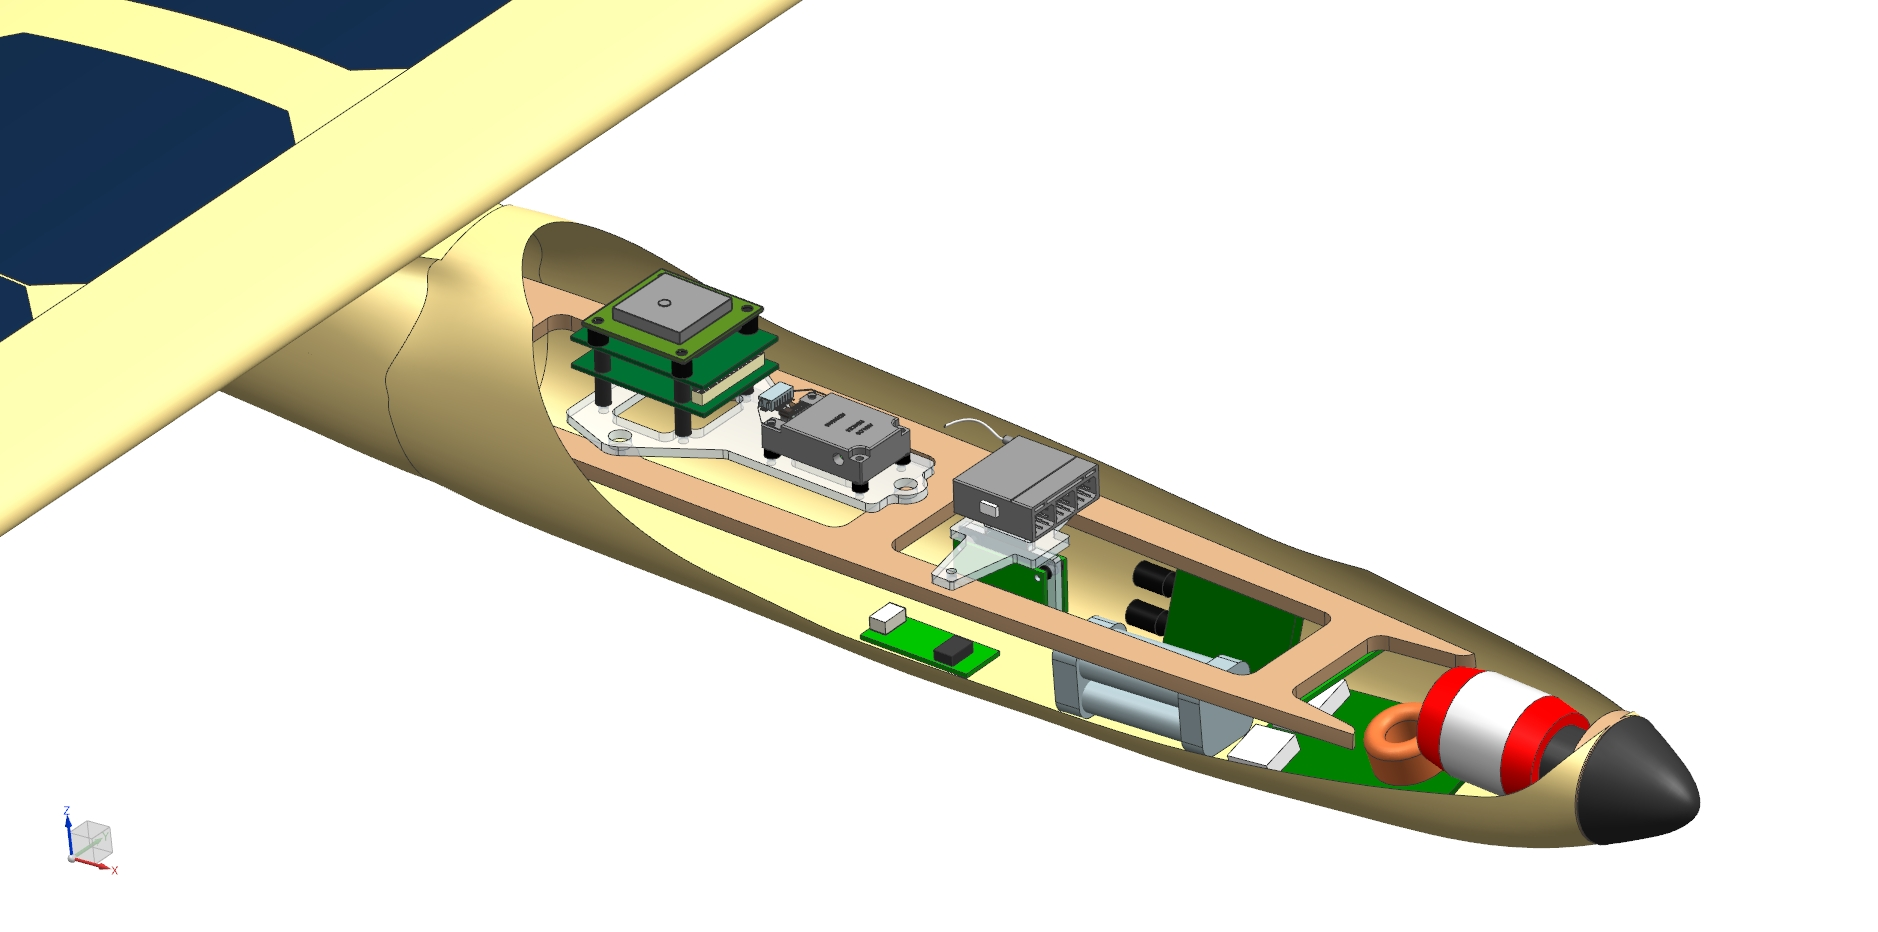
\includegraphics[width=\linewidth]{images/9_CAD_AtlantikSolarAvionics}
    \caption{Avionics components and their placement inside AtlantikSolar.}
    \label{fig:9_CAD_AtlantikSolarAvionics}
\end{figure}

\subsubsection{Payload}
% [THOMAS]
  - VI Sensor [ref to VI-sensor paper; ref to Leutenegger thesis?]
  - ~5 sentences + 1 picture
  
\subsection{State Estimation and Control Design}
Onboard state estimation \& control
\subsubsection{State estimation}
% [AMIR]
  - brief (5 sentence) description of SE type/principle
  - one verification plot (e.g. gps position ``ground truth'' vs. estimated position) 
  then REF to stefan\&Amir paper

\subsubsection{System Identification}
%[DR. ALEXIS]
 - System Identification \& Modelling
 
 \subsubsection{Control}
 %[PHILIPP writes this, DR. ALEXIS checks this]
 - Control using PID,  outer loops TECS \& L1 (Ref to OMLAS MED paper, also saying that there is future technologies which are being developed).
 - Full pre-flight verification in HIL
 
\subsection{Preliminary Results}
%[PHILIPP]
%if not in the sections before
  - control:   - SE\&Control: PID performance over various trim points. PID computational requirements (low!)
  - state estimation
  - solar system functioning
   - power efficiency curves. P\_level from Test flights.
   - potentially comparison to conceptual design 
   	- power (why not optimal: e.g. because optimal CD/CL\^1.5 assumed, but this has a) to be met in average and b) even then fluctuations as seen in flight tests are on the order of 2-3 degrees in AOA or +/- 1m/s, so this will never be met perfectly.
   	- actual mass vs. mass models?
